% !TeX program = pdflatex
\documentclass[11pt,a4paper]{article}
\usepackage[T1]{fontenc}
\usepackage[utf8]{inputenc}
\usepackage{lmodern}
\usepackage{geometry}
\geometry{margin=1in}
\usepackage{amsmath,amssymb,mathtools}
\usepackage{bm}
\usepackage{graphicx}
\usepackage{hyperref}
\usepackage{siunitx}

\title{Reduced Optimal Control with PDE Constraint:\\Model, Discretization, and First-Order Methods}
\author{Fachseminar}
\date{\today}

\begin{document}
\maketitle

\begin{abstract}

\end{abstract}

\section{Problem Statement}
We consider a linear-quadratic optimal control problem governed by the Poisson equation on a polygonal domain \(\Omega\subset\mathbb{R}^2\) (in computations, typically \([0,1]^2\)). A circular subregion \(\omega\subset\Omega\) is tagged on the mesh and serves as the support of the control. The control acts as a volumetric source term restricted to \(\omega\):
\begin{align}
  -\Delta y &= \chi_{\omega}\, u \quad\text{in } \Omega,\\
  y &= 0 \quad\text{on } \partial\Omega,
\end{align}
where \(\chi_{\omega}\) denotes the characteristic function of \(\omega\). We denote by \(V=H_0^1(\Omega)\) the state space and by \(U=L^2(\Omega)\) the control space. For a given target \(y_d\in L^2(\Omega)\) and a regularization parameter \(\beta>0\), we minimize
\begin{equation}
  J(y,u) = \tfrac12 \int_{\Omega} (y - y_d)^2\,dx + \tfrac{\beta}{2} \int_{\Omega} u^2\,dx.
\end{equation}
The target is chosen as the pyramid-like profile
\begin{equation}
  y_d(x) = 0.5 - \max\big(|x_1-0.5|,\,|x_2-0.5|\big),
\end{equation}
which belongs to \(L^2(\Omega)\). The control enters only on \(\omega\) via \(\chi_{\omega}\), so the effective source equals \(u\) on \(\omega\) and vanishes on \(\Omega\setminus\omega\). The PDE with homogeneous Dirichlet boundary conditions is well-posed for \(u\in L^2(\Omega)\), yielding a unique weak solution \(y\in V\) by Lax--Milgram.

\begin{figure}[ht]
  \centering
  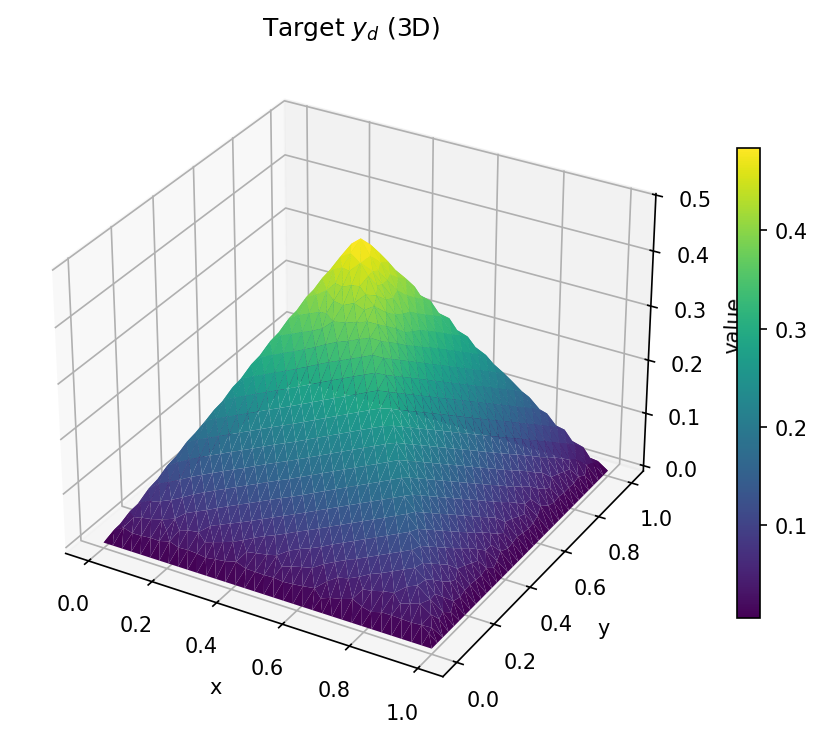
\includegraphics[width=0.75\linewidth]{../plots/y_d_3d.png}
  \caption{3D surface of the target profile $y_d$ on $\Omega$.}
  \label{fig:yd3d}
\end{figure}

\section{Variational Formulation and Discretization}
\paragraph{Weak formulation.} Define the bilinear and linear forms
\begin{align}
  a(y,v) &= \int_{\Omega} \nabla y\cdot\nabla v\, dx, & b(u,v) &= \int_{\omega} u\, v\, dx.
\end{align}
For any \(u\in L^2(\Omega)\), the weak state equation reads: find \(y\in V\) such that
\begin{equation}
  a(y,v) = b(u,v) \quad \forall v\in V.
\end{equation}
By coercivity of \(a(\cdot,\cdot)\) on \(V\) and boundedness of \(b(\cdot,\cdot)\), this admits a unique \(y\in V\).

\paragraph{Finite elements.} 
Let \(\mathcal{T}_h\) be a conforming triangulation of \(\Omega\). We use the conforming P1 space \(V_h\subset V\) with nodal basis \(\{\varphi_i\}_{i=1}^{n}\). The control is represented in the same P1 basis but measured with the \(L^2\) inner product (``control metric''). We assemble the matrices
\begin{align}
  A_{ij} &= \int_{\Omega} \nabla \varphi_j\cdot\nabla \varphi_i\, dx, &
  M_{ij} &= \int_{\Omega} \varphi_j\, \varphi_i\, dx, &
  B_{ij} &= \int_{\omega} \varphi_j\, \varphi_i\, dx, &
  (M_U)_{ij} &= \int_{\Omega} \varphi_j\, \varphi_i\, dx.
\end{align}
Here, \(A\) is the stiffness matrix for state/adjoint solves, \(M\) is the state mass matrix used to weight the tracking term, $B$ maps control coefficients to the state RHS via restriction to \(\omega\), and $M_U$ is the control-space mass matrix defining the \(L^2\) inner product in \(U_h\).

\paragraph{Boundary conditions.} 
Homogeneous Dirichlet boundary conditions are imposed on the state/adjoint by modifying \(A\) and zeroing the RHS at boundary degrees of freedom when solving. Importantly, no boundary conditions are applied to \(B\) or $M_U$; these operators remain the unmodified \(L^2\)-based forms on \(\Omega\).

\paragraph{Discrete state equation and objective.} 
With coefficient vectors \(\mathbf{y},\mathbf{u}\in\mathbb{R}^n\) and target coefficients \(\mathbf{y}_d\in\mathbb{R}^n\), the discrete state equation and cost read
\begin{align}
  A\, \mathbf{y} &= B\, \mathbf{u}, \\
  J(\mathbf{y},\mathbf{u}) &= \tfrac12 (\mathbf{y}-\mathbf{y}_d)^\top M (\mathbf{y}-\mathbf{y}_d) + \tfrac{\beta}{2} \mathbf{u}^\top MU\, \mathbf{u}.
\end{align}

\begin{figure}[ht]
  \centering
  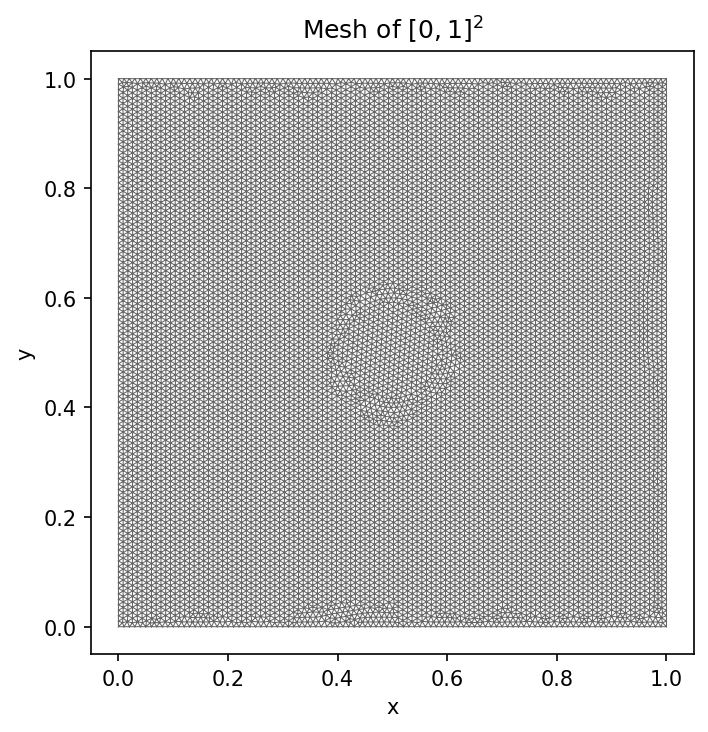
\includegraphics[width=0.7\linewidth]{../plots/mesh.png}
  \caption{Triangular mesh of $\Omega$ used for the P1 finite element discretization.}
  \label{fig:mesh}
\end{figure}

\section{Reduced Formulation}
\paragraph{State elimination.} Eliminating the state via the discrete PDE constraint gives \(\mathbf{y}(\mathbf{u})=A^{-1}B\,\mathbf{u}\) and the reduced functional \(F\colon\mathbb{R}^n\to\mathbb{R}\):
\begin{equation}
  F(\mathbf{u}) = \tfrac12 \big(A^{-1} B\, \mathbf{u} - \mathbf{y}_d\big)^\top M \big(A^{-1} B\, \mathbf{u} - \mathbf{y}_d\big) + \tfrac{\beta}{2}\, \mathbf{u}^\top MU\, \mathbf{u}.
\end{equation}

\paragraph{Adjoint and gradient (continuous view).} Introducing an adjoint variable \(p\in V\) and the Lagrangian
\begin{equation}
  \mathcal{L}(y,u,p) = \tfrac12\|y-y_d\|_{L^2(\Omega)}^2 + \tfrac{\beta}{2}\|u\|_{L^2(\Omega)}^2 + a(y,p) - b(u,p),
\end{equation}
the optimality system reads: state \(a(y,v)=b(u,v)\), adjoint \(a(v,p)=(y-y_d,v)\) for all \(v\in V\), and variational gradient condition \((\beta u + \chi_{\omega} p, w)_{L^2(\Omega)}=0\) for all \(w\in U\). Hence, formally, \(\beta u + p\,\chi_{\omega}=0\) in \(\Omega\).

\paragraph{Adjoint and gradient (discrete view).} In coefficients, the adjoint solves
\begin{equation}
  A\, \mathbf{p} = M\, (\mathbf{y}(\mathbf{u}) - \mathbf{y}_d),
\end{equation}
and the gradient with respect to the control space inner product induced by \(MU\) is
\begin{equation}
  \nabla F(\mathbf{u}) = MU^{-1}\, B^\top \mathbf{p} + \beta\, \mathbf{u}.
\end{equation}
The first-order optimality condition \(\nabla F(\mathbf{u}_*)=0\) is equivalent to
\begin{equation}
  B^\top \mathbf{p}_* + \beta\, MU\, \mathbf{u}_* = 0, \qquad A\, \mathbf{p}_* = M\, (\mathbf{y}(\mathbf{u}_*)-\mathbf{y}_d).
\end{equation}

\paragraph{Hessian, convexity, and Lipschitz constant.} The reduced Hessian applied to \(\mathbf{v}\) is
\begin{equation}
  H\, \mathbf{v} = MU^{-1}\, B^\top A^{-1} M A^{-1} B\, \mathbf{v} + \beta\, \mathbf{v}.
\end{equation}
Since \(A\), \(M\), and \(MU\) are symmetric positive definite on their natural subspaces and \(B\) is linear, the quadratic form associated with \(H\) is strictly positive for \(\beta>0\); thus, \(F\) is strictly convex with a unique minimizer. In the \(U\)-metric, the gradient is Lipschitz with constant
\begin{equation}
  L = \big\| MU^{-1/2} B^\top A^{-1} M A^{-1} B\, MU^{-1/2} \big\|_2 + \beta,
\end{equation}
namely the spectral radius of the SPD term plus \(\beta\).

\end{document}